\documentclass[11pt,border=4pt]{standalone}
% Estilo comum dos fluxogramas do Caderno C3 (cores do modelo do MOP)
\usepackage[T1]{fontenc}
\usepackage[utf8]{inputenc}
\usepackage{helvet}
\renewcommand{\familydefault}{\sfdefault}
\usepackage{amssymb}
\usepackage{tikz}
\usetikzlibrary{positioning, arrows.meta, shapes.geometric, shapes.symbols, shapes.misc,
  calc, fit, backgrounds, decorations.pathmorphing, patterns, shadows}
% Paleta do modelo do caderno
\definecolor{cTeal}{HTML}{00747A}
\definecolor{cNavy}{HTML}{0B3A5A}
\definecolor{cBlue}{HTML}{0A73BA}
\definecolor{cBlueBg}{HTML}{EBF4F9}
\definecolor{cTealBg}{HTML}{E3F1F2}
\definecolor{cTealMid}{HTML}{9CCFD2}
\definecolor{cGrayBg}{HTML}{F2F2F2}
\definecolor{cGrayLine}{HTML}{BFBFBF}
\definecolor{cGrayText}{HTML}{595959}
\definecolor{cText}{HTML}{1A1A1A}
\definecolor{cAmber}{HTML}{B7791F}
\definecolor{cAmberBg}{HTML}{FDF3DC}
\definecolor{cGreen}{HTML}{3D7D3A}
\definecolor{cGreenBg}{HTML}{E8F2E4}
\color{cText}
\tikzset{
  every node/.style={font=\footnotesize, text=cText},
  etapa/.style={draw=cTeal, fill=cTealBg, rounded corners=2pt, align=center,
     inner sep=3.5pt, minimum height=0.85cm, text width=#1, line width=0.6pt},
  etapa/.default={3.2cm},
  marco/.style={draw=cNavy, fill=cNavy, rounded corners=2pt, align=center,
     inner sep=3.5pt, minimum height=0.85cm, text width=#1,
     font=\footnotesize\bfseries, text=white},
  marco/.default={3.2cm},
  marcoteal/.style={draw=cTeal, fill=cTeal, rounded corners=2pt, align=center,
     inner sep=3.5pt, minimum height=0.85cm, text width=#1,
     font=\footnotesize\bfseries, text=white},
  marcoteal/.default={3.2cm},
  externo/.style={draw=cGrayLine, fill=cGrayBg, rounded corners=2pt, align=center,
     inner sep=3.5pt, minimum height=0.85cm, text width=#1},
  externo/.default={3.2cm},
  produto/.style={draw=cTeal!70, fill=white, rounded corners=1pt, align=center,
     inner sep=2.5pt, minimum height=0.6cm, text width=#1, font=\scriptsize},
  produto/.default={2.4cm},
  decisao/.style={draw=cAmber, fill=cAmberBg, diamond, aspect=2, align=center,
     inner sep=1pt, font=\scriptsize, line width=0.6pt},
  correcao/.style={draw=cAmber, fill=cAmberBg, rounded corners=2pt, align=center,
     inner sep=3pt, minimum height=0.8cm, text width=#1, font=\scriptsize},
  correcao/.default={2.6cm},
  transversal/.style={draw=cBlue, fill=cBlueBg, dashed, rounded corners=2pt, align=center,
     inner sep=3.5pt, text width=#1, line width=0.6pt},
  transversal/.default={6cm},
  seta/.style={-{Stealth[length=2.2mm,width=1.8mm]}, line width=0.8pt, draw=cNavy},
  setaleve/.style={-{Stealth[length=1.8mm,width=1.5mm]}, line width=0.6pt, draw=cGrayText},
  setatracejada/.style={-{Stealth[length=2mm]}, line width=0.7pt, dashed, draw=cGrayText},
  rotulo/.style={font=\scriptsize\itshape, text=cGrayText, fill=white, inner sep=1pt},
  fase/.style={signal, signal to=east, signal from=west, draw=cTeal, fill=cTealBg,
     align=center, font=\scriptsize\bfseries, minimum height=1.05cm, text width=#1,
     inner sep=2pt},
  fase/.default={1.9cm},
  raia/.style={draw=cGrayLine, fill=cGrayBg, minimum width=#1, minimum height=0.9cm,
     anchor=north west},
  tituloraia/.style={font=\scriptsize\bfseries, text=cNavy, align=center, text width=1.75cm},
  cab/.style={font=\scriptsize\bfseries, text=white, fill=cNavy, align=center,
     inner sep=3pt, text width=#1, minimum height=0.6cm},
  cab/.default={3cm},
  bloco/.style={draw=cGrayLine, fill=cGrayBg, rounded corners=3pt},
}
% sem hifenização nas caixas dos fluxogramas
\AtBeginDocument{\hyphenpenalty=10000 \exhyphenpenalty=10000 \sloppy}

\begin{document}

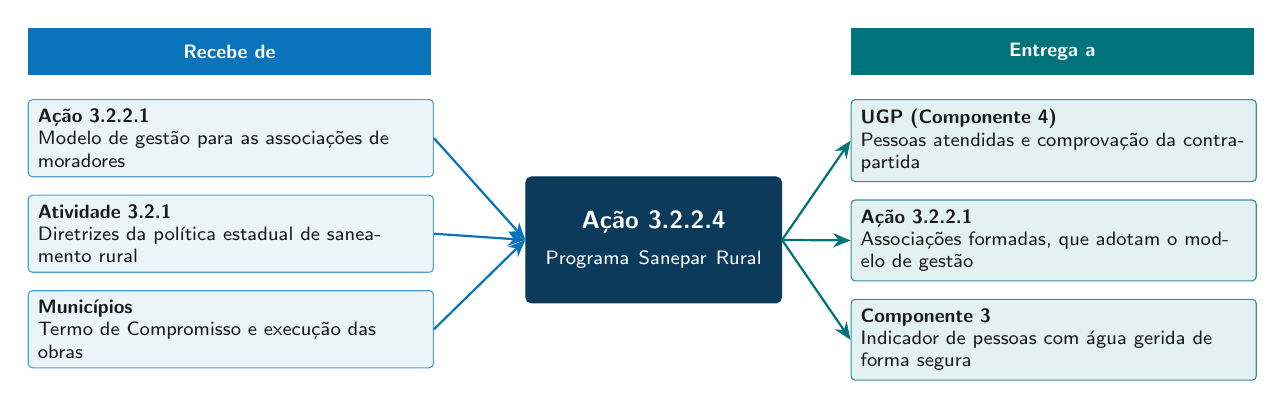
\begin{tikzpicture}

  \tikzset{
    rec/.style={draw=cBlue!70, fill=cBlueBg, rounded corners=1.5pt, align=left,
      text width=4.9cm, inner sep=3.5pt, font=\scriptsize, minimum height=0.95cm},
    ent/.style={draw=cTeal!80, fill=cTealBg, rounded corners=1.5pt, align=left,
      text width=4.9cm, inner sep=3.5pt, font=\scriptsize, minimum height=0.95cm}
  }
  \node[cab=4.9cm, fill=cBlue, anchor=north west] (hR) at (0,0) {Recebe de};
  \node[cab=4.9cm, fill=cTeal, anchor=north west] (hE) at (10.45,0) {Entrega a};

  \node[rec, below=0.3cm of hR.south west, anchor=north west] (r1) {\textbf{Ação 3.2.2.1}\\ Modelo de gestão para as associações de moradores};
  \node[rec, below=0.22cm of r1] (r2) {\textbf{Atividade 3.2.1}\\ Diretrizes da política estadual de saneamento rural};
  \node[rec, below=0.22cm of r2] (r3) {\textbf{Municípios}\\ Termo de Compromisso e execução das obras};
  \node[ent, below=0.3cm of hE.south west, anchor=north west] (s1) {\textbf{UGP (Componente 4)}\\ Pessoas atendidas e comprovação da contrapartida};
  \node[ent, below=0.22cm of s1] (s2) {\textbf{Ação 3.2.2.1}\\ Associações formadas, que adotam o modelo de gestão};
  \node[ent, below=0.22cm of s2] (s3) {\textbf{Componente 3}\\ Indicador de pessoas com água gerida de forma segura};

  \path let \p1=(r1.north), \p2=(r3.south), \p3=(s1.north), \p4=(s3.south) in
    coordinate (cc) at (7.95, {(max(\y1,\y3)+min(\y2,\y4))/2});
  \node[marco=3.0cm, minimum height=1.6cm, font=\small\bfseries] (A) at (cc) {Ação 3.2.2.4\\[2pt]
    \normalfont\scriptsize Programa Sanepar Rural};
  \draw[seta, draw=cBlue] (r1.east) -- (A.west);
  \draw[seta, draw=cBlue] (r2.east) -- (A.west);
  \draw[seta, draw=cBlue] (r3.east) -- (A.west);
  \draw[seta, draw=cTeal] (A.east) -- (s1.west);
  \draw[seta, draw=cTeal] (A.east) -- (s2.west);
  \draw[seta, draw=cTeal] (A.east) -- (s3.west);
\end{tikzpicture}

\end{document}
